\documentclass{beamer}

\mode<presentation> {
  \usetheme{Dresden}
  \usecolortheme{beaver}
  \setbeamercovered{transparent}
  \setbeamercolor*{item}{fg=darkred}
  \setbeamercolor*{block title}{fg=darkred}
}

\usepackage{ucs}
\usepackage[utf8x]{inputenc}
\usepackage[czech]{babel}
\usepackage{palatino}
\usepackage{graphicx}
\usepackage{listings}
\lstset{basicstyle=\sffamily\footnotesize,breaklines=true,language=tex}

\title{Linux Kernel Networking}
\author{Josef Luštický}
\institute{iXperta s.r.o}
\date{24.~4.~2015}

\begin{document}

\begin{frame}
  \titlepage
\end{frame}

% Numbering
\expandafter\def\expandafter\insertshorttitle\expandafter{%
  \insertshorttitle\hfill%
  \insertframenumber\,/\,\inserttotalframenumber}

% Do not count the Titlepage in frame numbers
\addtocounter{framenumber}{-1}

\begin{frame}{Obsah}
	\begin{itemize}
		\item Ethernet
		\item 10~GbE, 40/100~GbE
		\item Původní zpracování paketů
		\item Nestíháme - New API (NAPI)
		\item Delegujme práci na hardware - Offloads
		\item Vícejádrové CPU - škálování
		\item Diskuse, procházení kódu, možnosti nastavení, ...
	\end{itemize}
\end{frame}

\begin{frame}{Ethernet 1980 - IEEE 1983}
	\begin{itemize}
		\item Původně 10~Mbit přes Coax
		\item 10~BASE-T - kroucená dvojlinka
			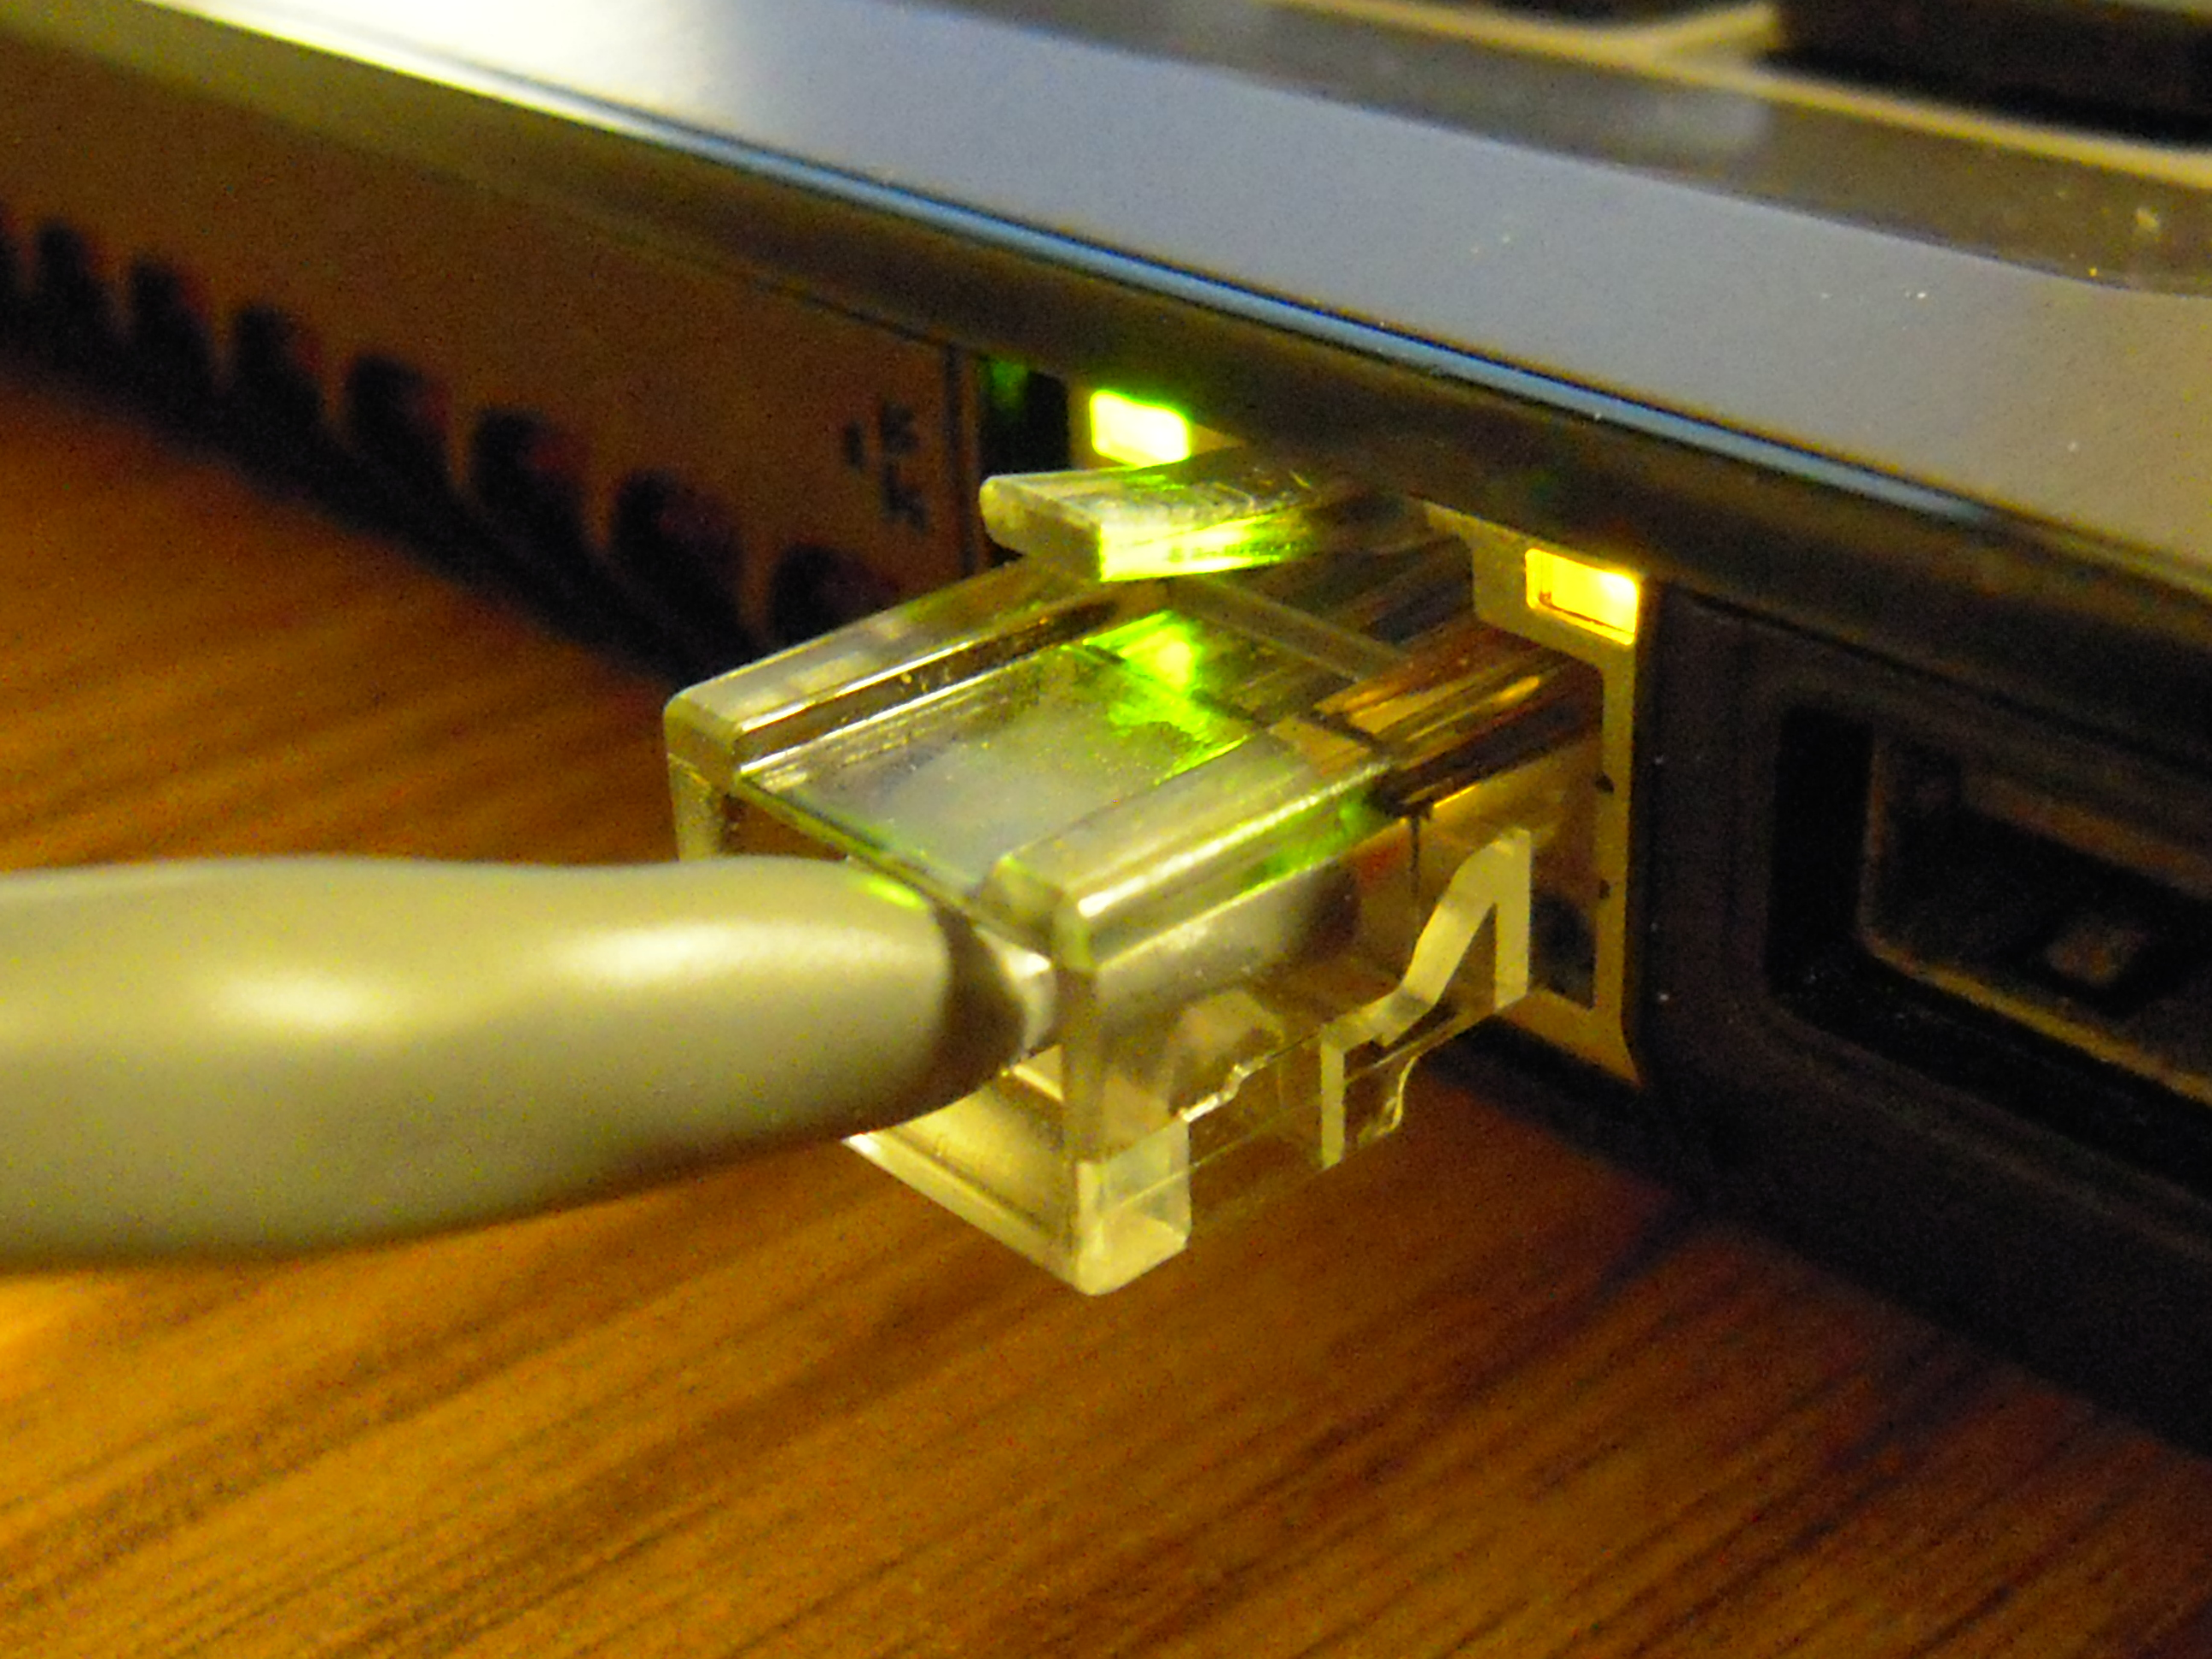
\includegraphics[width=2.5cm,keepaspectratio]{fig/rj45.jpg}
		\item Rámce 84 až 1538 bajtů (až 14~880 fps)
	\end{itemize}
	\centering
	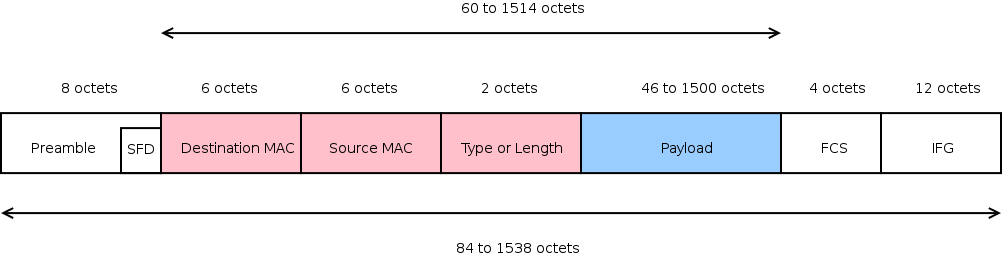
\includegraphics[width=9cm,keepaspectratio]{fig/ethernet-frame.png}
\end{frame}

\begin{frame}{Ethernet dnes}
	100~Mbit
	\begin{itemize}
		\item 148~800~fps při 84~B (8~100 při 1536~B)
		\item 500~MHz CPU 3~400 taktů na zpracování rámce (6.7 micro~s)
	\end{itemize}
	1~Gbit
	\begin{itemize}
		\item až 1.48 Mpps, tj. každých 670~ns další rámec
		\item 2~GHz CPU má k dispozici 1~351 taktů
	\end{itemize}
\end{frame}

\begin{frame}{Velikost rámců v AMS-IX}
	\centering
	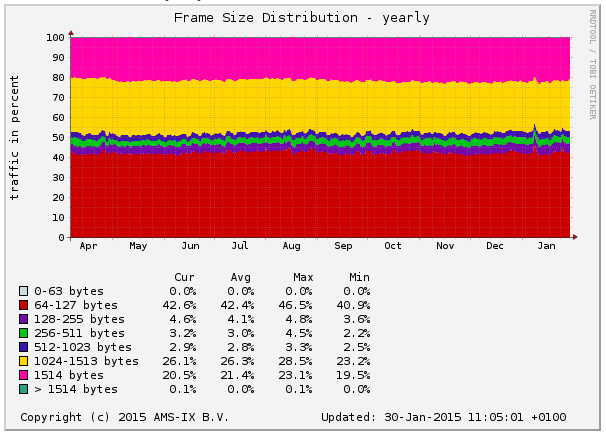
\includegraphics[width=8cm,keepaspectratio]{fig/amsix.png} \\
	Průměrná velikost rámce v Internetu 760~B
\end{frame}

\begin{frame}{10~GbE a 40~GbE}
	10~GbE
	\begin{itemize}
		\item 10~GBASE-T dnes už levnější než optické spoje
	\end{itemize}
	40~GbE
	\begin{itemize}
		\item Frame rates - 3.26 - 59.5~Mpps (MTU 1518 / 64~B) \\
		307.6 / 16.8~ns (51 cyklů na 3~GHz CPU)
		\item Propustnost - 4.6~GB/s (PCIe 3.0 x8 zvládne 7.9~GB/s)
		\item Plánovaný 40~GBASE-T s dosahem 30~m
	\end{itemize}
	\begin{figure}
		\centering
		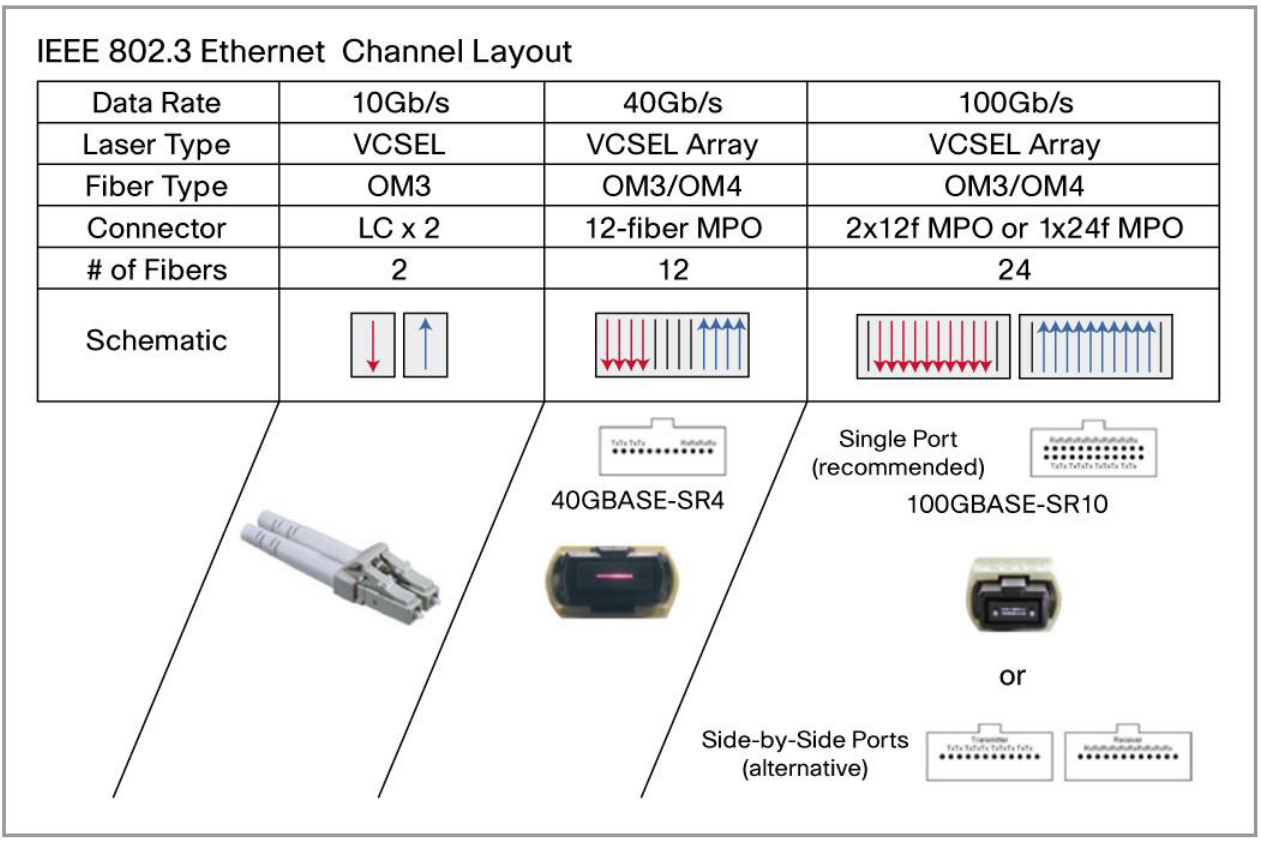
\includegraphics[width=6cm,keepaspectratio]{fig/ethernet-layout.png}
	\end{figure}
\end{frame}

\begin{frame}{OS GNU/Linux}
	\centering
	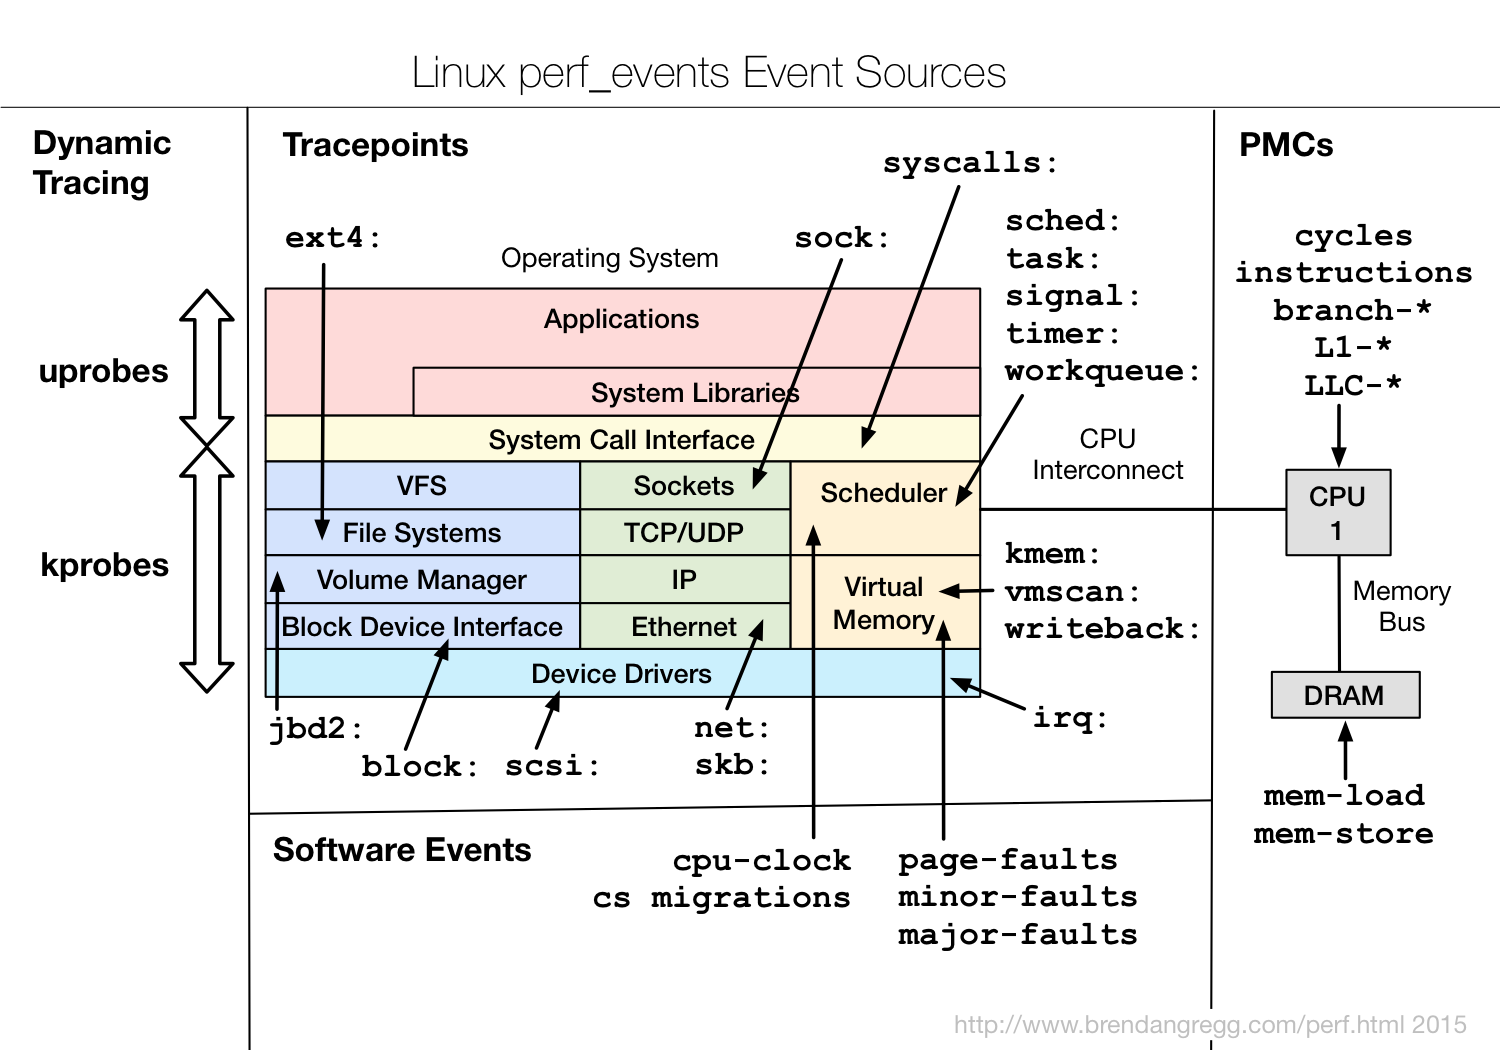
\includegraphics[width=8cm,keepaspectratio]{fig/perf_events_map.png}
	\begin{itemize}
		\item Uživatelský kontext
		\item Kontext přeřušení (hard IRQ)
	\end{itemize}
\end{frame}

\begin{frame}{Síťový stack v Linuxu}
	\begin{figure}
		\centering
		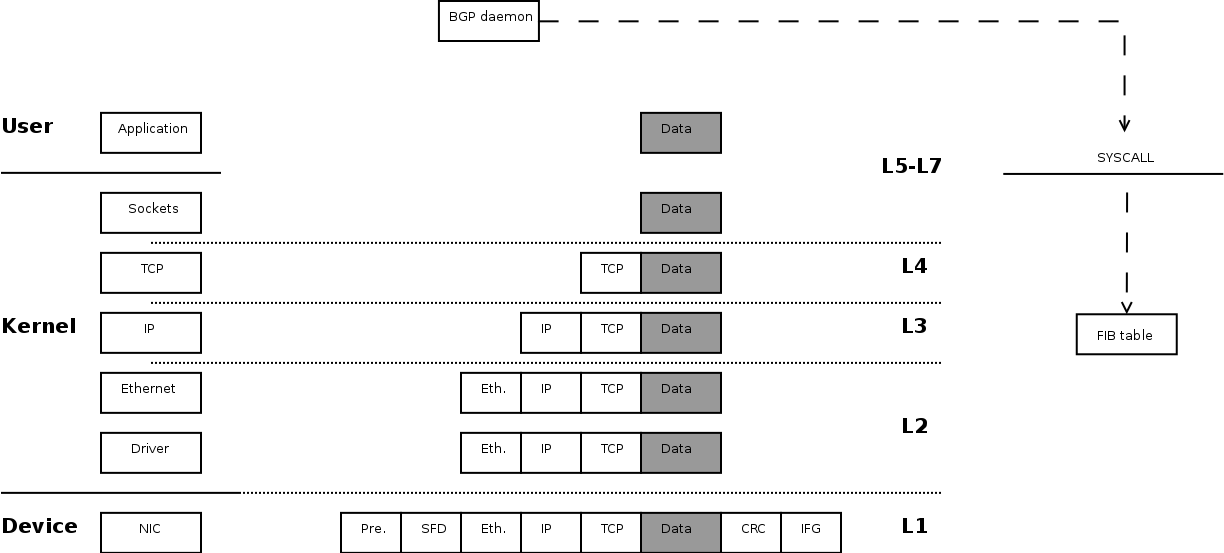
\includegraphics[width=8cm,keepaspectratio]{fig/layers.png}
	\end{figure}
\end{frame}

\begin{frame}{Linux - zdrojové kódy}
	\begin{itemize}
		\item arch/ arm, x86, mips, um
		\item fs/ ext2, reiserfs, btrfs, proc, sysfs, debugfs
		\item mm/ "Memory Management"
		\item net/ bluetooth, ethernet, ipv4, ipv6
		\item drivers/ net/ ethernet, usb, wireless 
		\item Documentation/
	\end{itemize}
\end{frame}

\begin{frame}{L3 - IPv4 stack}
	\begin{figure}
		\centering
		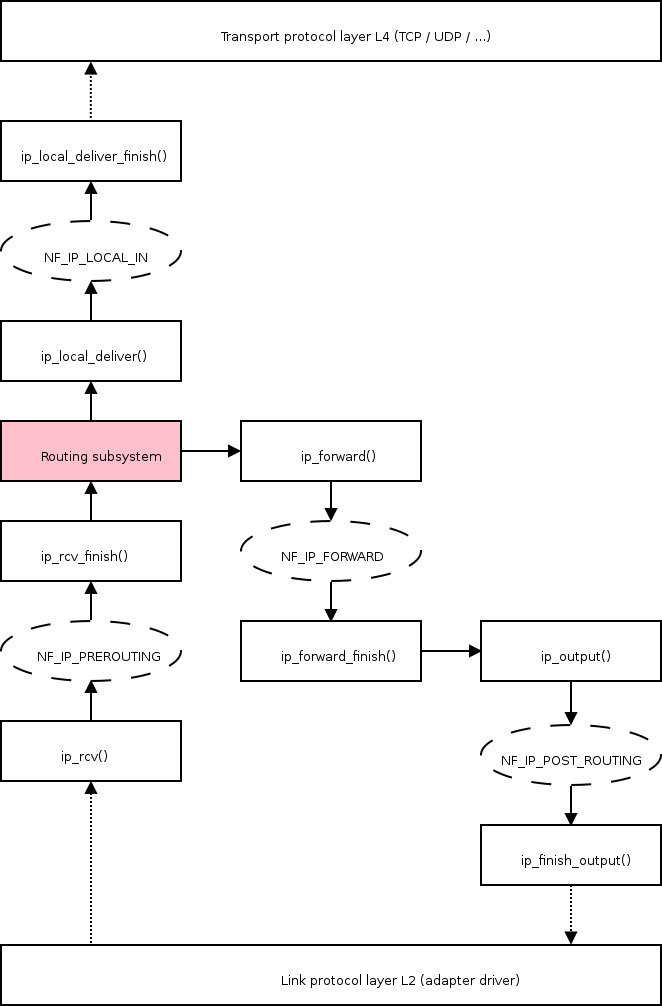
\includegraphics[width=6cm,height=6.5cm]{fig/kernel-layer3-flow.png}
	\end{figure}
\end{frame}

\begin{frame}{Reprezentace paketu - sk\_buff}
	\begin{figure}
		\centering
		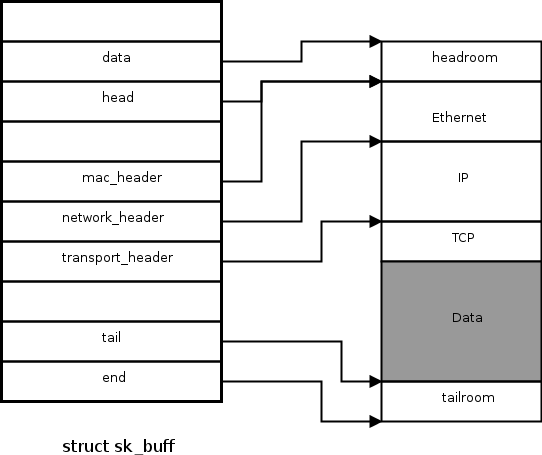
\includegraphics[width=6cm,keepaspectratio]{fig/skb.png}
	\end{figure}
\end{frame}


\begin{frame}{L2 - ovladače}
	\begin{itemize}
		\item API ovladačů - virtuální funkce
		\item Ovladač alokuje buffer pro přenos paketů
		\item DMA přenosy do bufferu
	\end{itemize}
\end{frame}

\begin{frame}{Původní zpracování paketů - Kernel 2.4}
	\begin{itemize}
		\item DMA přenos do ring bufferu
		\item Přerušení IRQ - rutina provede nejnutnější práci
		\begin{itemize}
			\item Inicializace sk\_buff
			\item Aktualizace statistik
			\item Naplánování NET\_RX\_SOFTIRQ
		\end{itemize}
		\item Zpracování paketu v softirq - přidání do fronty CPU
	\end{itemize}
\end{frame}

\begin{frame}{Původní zpracování paketů - přehled}
	\centering
	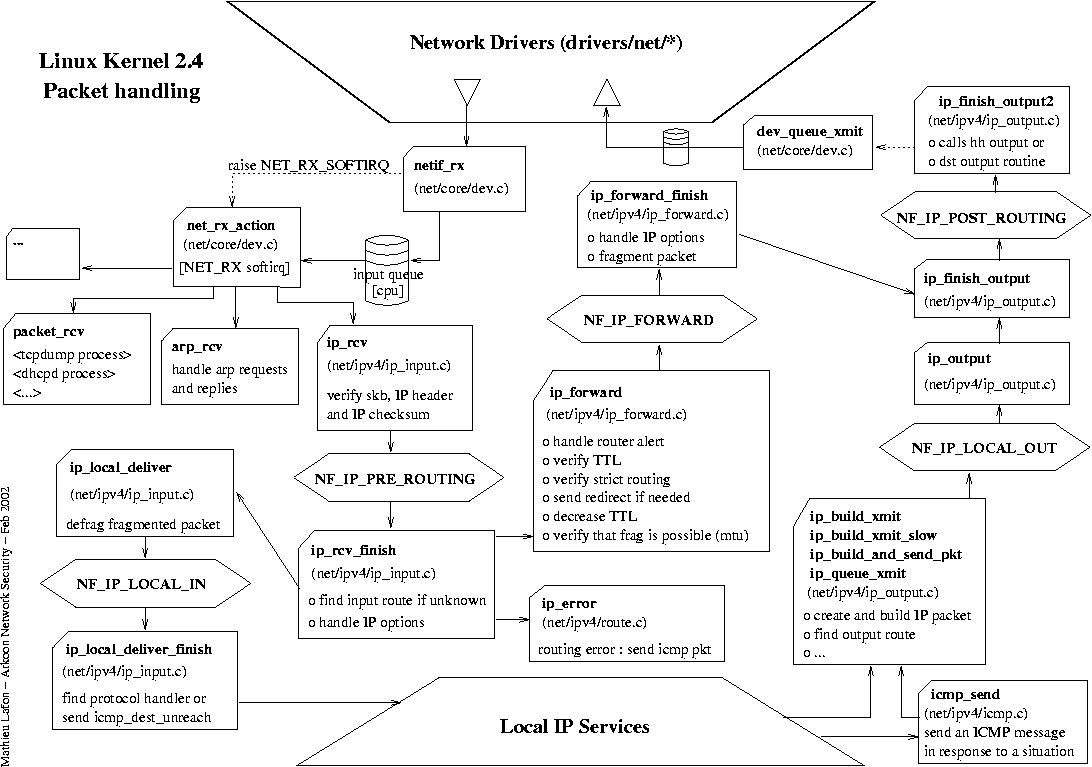
\includegraphics[width=10cm,keepaspectratio]{fig/kernel_24.png}
\end{frame}

\begin{frame}{100Mbit nestíháme - New API}
	\begin{itemize}
		\item Interrupt mitigation
		\item První paket způsobí přeřušení
		\item Další pakety kernel vyzvedává pakety ze síťové karty v rámci SoftIRQ
		\item Nutné úpravy ovladače a možnost vypnout přerušení
	\end{itemize}
\end{frame}

\begin{frame}{New API workflow}
	\centering
	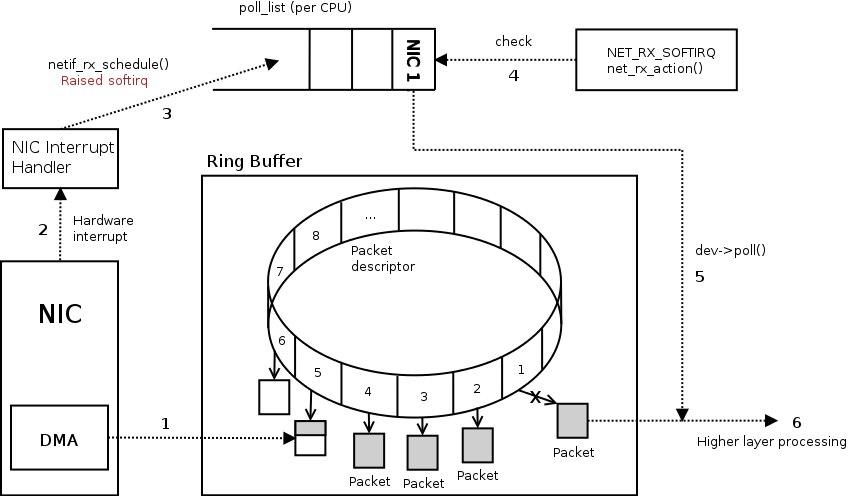
\includegraphics[width=10cm,keepaspectratio]{fig/napi-workflow.png}
\end{frame}

\begin{frame}{Delegujme práci na hardware}
	\begin{itemize}
		\item Kontrolní součty
		\item Fragmentace IP
		\item Segmentace TCP
		\item Scatter-Gather - DMA přenos z více míst
		\item TCP Offload Engine - ACK, otevírání a uzavírání spojení
	\end{itemize}
\end{frame}

\begin{frame}{Generic Receive Offload - varianta bez GRO}
	\centering
	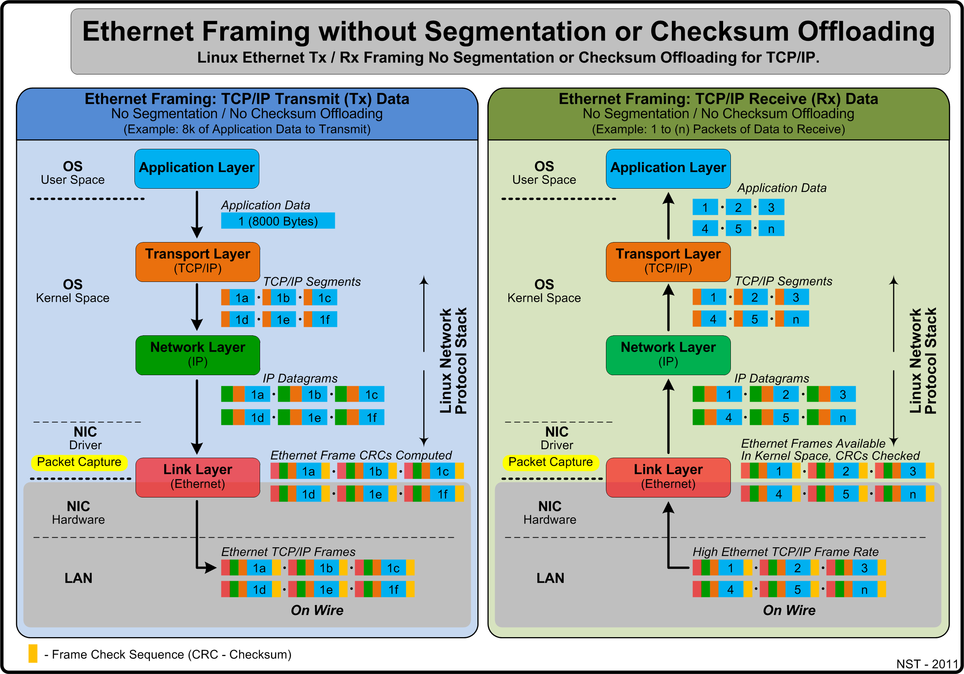
\includegraphics[width=10cm,keepaspectratio]{fig/no_segmentation_offloading.png}
\end{frame}

\begin{frame}{Generic Receive Offload - varianta s GRO}
	\centering
	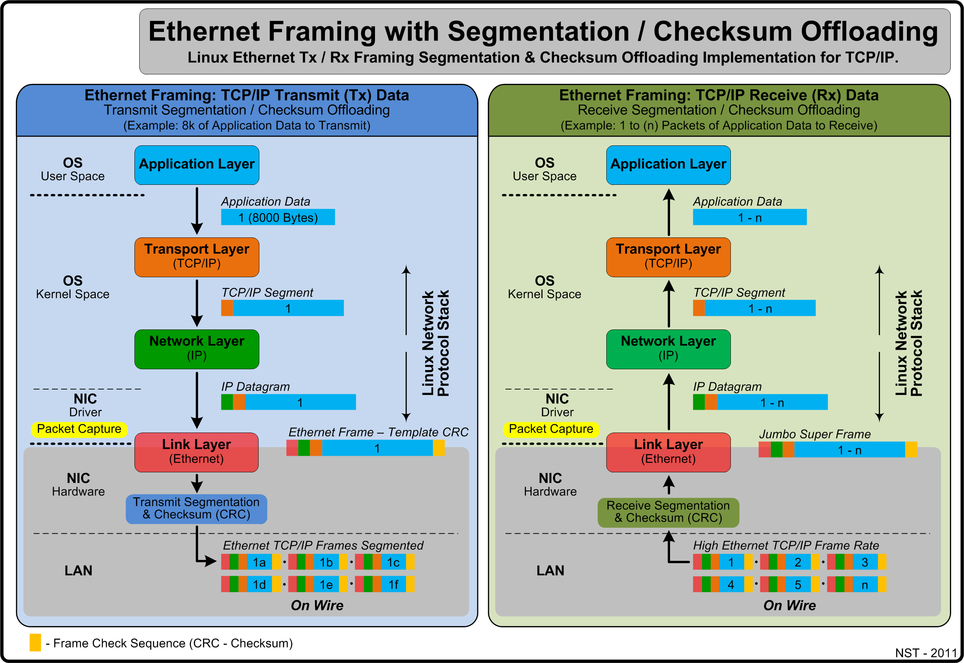
\includegraphics[width=10cm,keepaspectratio]{fig/segmentation_offloading.png}
\end{frame}

\begin{frame}[fragile]{Konfigurace Offload mechanismů}
	Zobrazení
	\begin{lstlisting}
		ethtool --show-offload eth0
	\end{lstlisting}
	Nastavení
	\begin{lstlisting}
		ethtool --offload eth0 rx on
	\end{lstlisting}
	Ovladač implementuje ethtool\_ops
\end{frame}

\begin{frame}{Růst výkonu sítí a CPU}
	\centering
	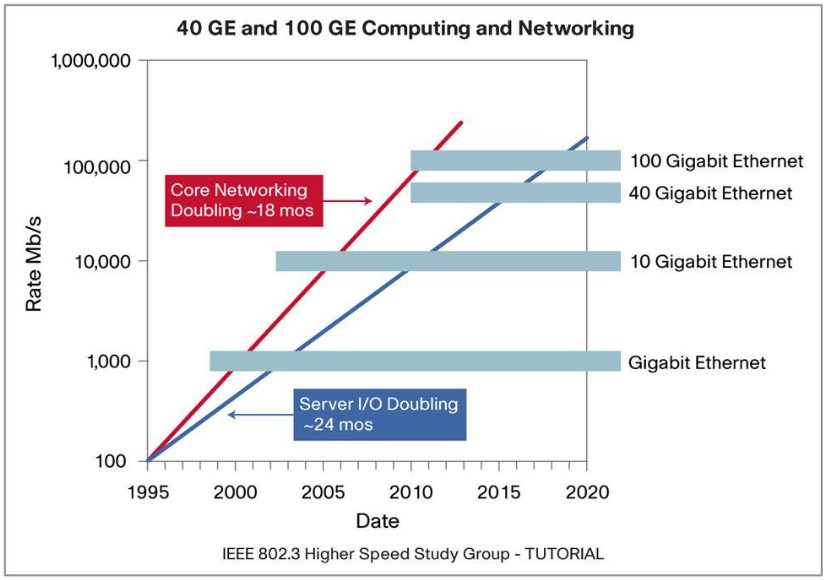
\includegraphics[width=9cm,keepaspectratio]{fig/performance-gap.png}
\end{frame}

\begin{frame}{Vícejádrové CPU - škálování - kernel 2.6.35}
	\begin{itemize}
		\item Škálování založeno různých síťových tocích - Hash nad hlavičkami
		\item Každé CPU může zpracovávat jiné toky
		\item Receive Packet Steering (RPS) - určení CPU softwarem
		\item Receive Side Steering (RSS) - určení CPU síťovou kartou pomocí přerušení (MSI-X)
		\item Vícefrontové síťové karty - Multiqueue NIC
	\end{itemize}
\end{frame}

\begin{frame}{Receive Side Scaling (RSS)}
	\centering
	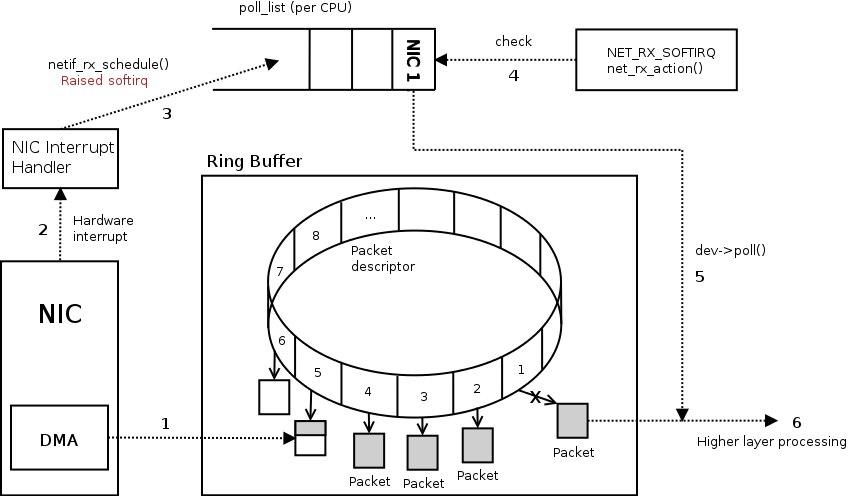
\includegraphics[width=3cm,keepaspectratio]{fig/napi-workflow.png} \\
	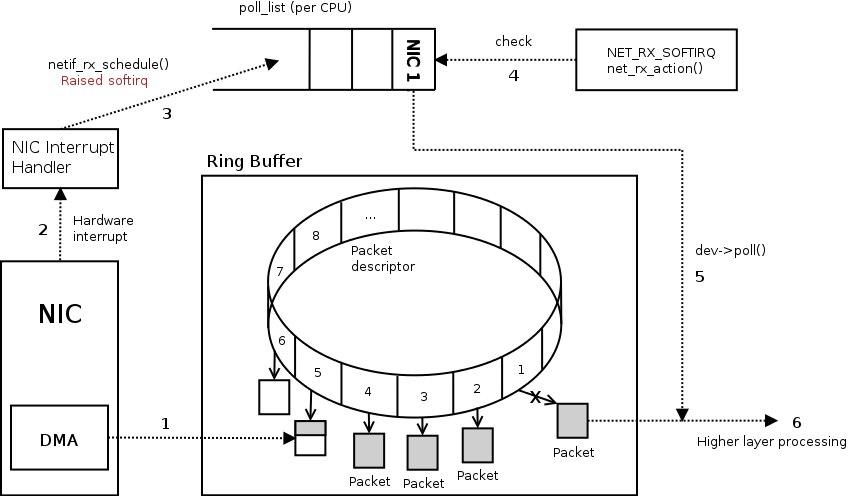
\includegraphics[width=3cm,keepaspectratio]{fig/napi-workflow.png} \\
	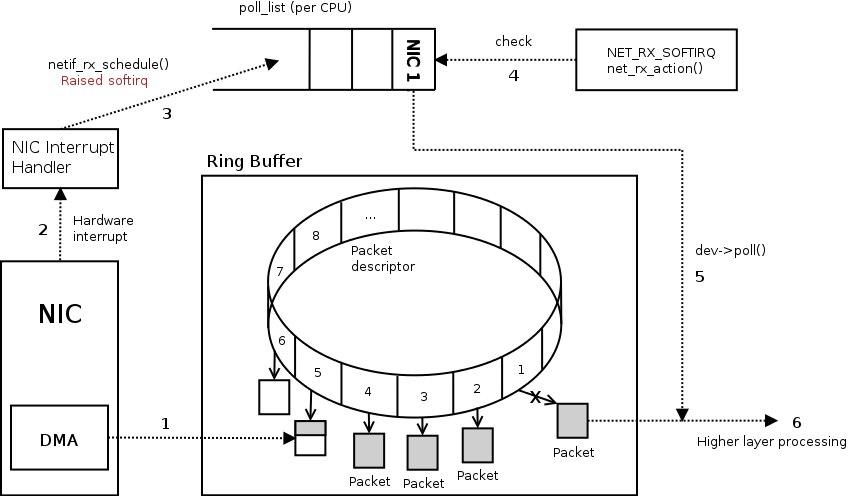
\includegraphics[width=3cm,keepaspectratio]{fig/napi-workflow.png} \\
	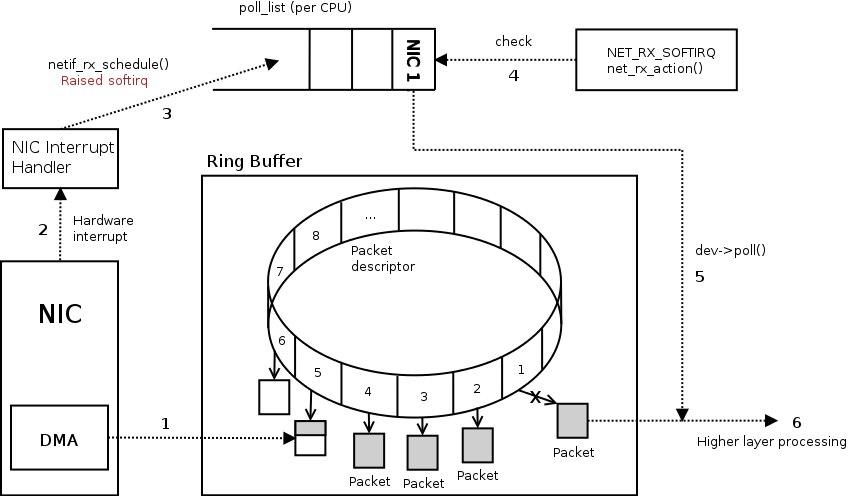
\includegraphics[width=3cm,keepaspectratio]{fig/napi-workflow.png}
\end{frame}

\begin{frame}[fragile]{Konfigurace RSS}
	Nastavení počtu front
	\begin{lstlisting}
		ethtool --show-channels eth0
		ethtool --set-channels eth0 rx 4
	\end{lstlisting}
	Mapování pomocí IRQ affinity
	\begin{lstlisting}
		cat /proc/interrupts
		echo "0-1,4" > /proc/irq/32/smp_affinity_list
		echo "013" > /proc/irq/32/smp_affinity
	\end{lstlisting}
\end{frame}

\begin{frame}[fragile]{Transmit Packet Steering (XPS) - kernel 2.6.38}
	Určíme které procesory mohou využít danou TX frontu
	\begin{lstlisting}
		/sys/class/net/eth0/queues/tx-0/xps_cpus
	\end{lstlisting}

	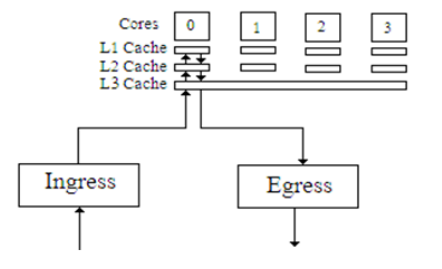
\includegraphics[width=5cm,keepaspectratio]{fig/irq-cache.png}
	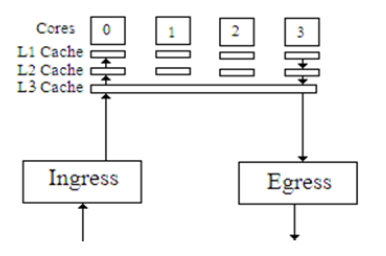
\includegraphics[width=5cm,keepaspectratio]{fig/irq-spread.png}
\end{frame}

\begin{frame}{Odesílání xmit\_more - kernel 3.19}
	Inspirace z blokových zařízení - nahrajeme pakety do ring bufferu, ale neodesíláme je
	\begin{itemize}
		\item Paket (sk\_buff - obsahuje příznak xmit\_more)
		\item Paket (sk\_buff - obsahuje příznak xmit\_more)
		\item ...
		\item Paket (sk\_buff - neobsahuje xmit\_more) - odeslání
	\end{itemize}
	pktgen zvládá generovat 14.88~Mpps
\end{frame}

\begin{frame}{Linux jako směrovač - Mellanox ConnectX-3 40~Gbps}
	\begin{itemize}
		\item 1 CPU HT zvládá 1~000~000 fps
		\item 8 CPU HT zvládá 5~800~000 fps (35.30~Gbps)
		\item Stále nezvládáme frame rate 14.88~Mpps
		\item Zpracování rámce na 1 CPU stále trvá dlouho (1 micro s)
	\end{itemize}
\end{frame}

\begin{frame}[fragile]{Co nás brzdí?}
	Memory management - alokace skb, zamykání, ...
	\begin{lstlisting}
	perf top -C 10
	  11.42%  [kernel]  [k] fib_table_lookup
	   9.62%  [kernel]  [k] _raw_spin_lock
	   6.65%  [kernel]  [k] mlx4_en_xmit
	   4.84%  [kernel]  [k] memcpy
	   4.03%  [kernel]  [k] mlx4_en_complete_rx_desc
	   3.61%  [kernel]  [k] check_leaf.isra.7
	   3.52%  [kernel]  [k] mlx4_en_free_tx_desc.isra.22
	   3.42%  [kernel]  [k] mlx4_en_process_rx_cq
	   3.16%  [kernel]  [k] mlx4_en_poll_tx_cq
	   2.89%  [kernel]  [k] put_compound_page
	   2.72%  [kernel]  [k] dev_queue_xmit
	\end{lstlisting}
\end{frame}

\end{document}
